\documentclass[border=1pt]{standalone}
\usepackage{tikz}

\begin{document}
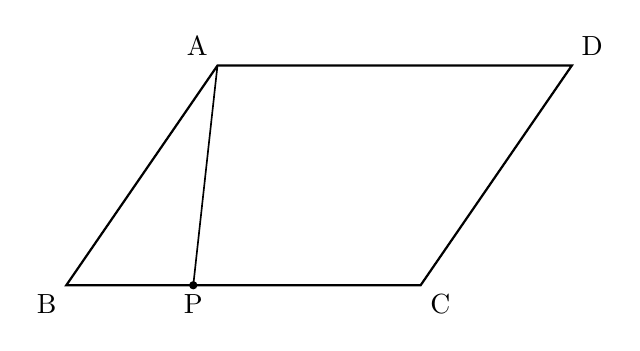
\begin{tikzpicture}

    % パラメータの定義
    \pgfmathsetmacro{\X}{4.5}
    \pgfmathsetmacro{\Y}{0.62*\X}

    \pgfmathsetmacro{\d}{1.28*\X/3}

    % 点の定義
    \coordinate (B) at (0,0);
    \coordinate (A) at (\d,\Y);
    \coordinate (D) at (\d+\X,\Y);
    \coordinate (C) at (\X,0);
    \coordinate (P) at (\d*0.84,0);
        
    % 点の描画
    \node at (B) [below left] {$\mathrm{B}$};
    \node at (A) [above left] {$\mathrm{A}$};
    \node at (D) [above right] {$\mathrm{D}$};
    \node at (C) [below right] {$\mathrm{C}$};
    \fill (P) circle (1.5pt) node [below] {$\mathrm{P}$};
    
    % 線分の描画        
    \draw [thick] (A) -- (B) -- (C) -- (D) -- cycle;
    \draw [semithick] (A) -- (P);

\end{tikzpicture}
\end{document}


